\documentclass[12pt,a4paper,onecolumn]{exam}

\usepackage{amsmath}
\usepackage{amsthm}
\usepackage{amssymb}
\usepackage{graphicx}
\usepackage{float}
\usepackage{geometry}
\usepackage{tikz}
\usepackage[skins]{tcolorbox}
\usepackage{listings}
\usepackage{xcolor}
\usepackage{hyperref}
\usepackage{multirow}
\usepackage{adjustbox}
\usepackage{booktabs}
\usepackage[font=small]{caption}
\usepackage{subcaption}

% --- Code Listing Colors ---
\definecolor{codegreen}{rgb}{0,0.6,0}
\definecolor{codegray}{rgb}{0.5,0.5,0.5}
\definecolor{codepurple}{rgb}{0.58,0,0.82}
\definecolor{backcolour}{rgb}{0.95,0.95,0.92}

% --- Code Listing Style ---
\lstdefinestyle{mystyle}{
    backgroundcolor=\color{backcolour},
    commentstyle=\color{codegreen},
    keywordstyle=\color{magenta},
    numberstyle=\tiny\color{codegray},
    stringstyle=\color{codepurple},
    basicstyle=\ttfamily\footnotesize,
    breaklines=true,
    captionpos=b,
    keepspaces=true,
    numbers=left,
    numbersep=2pt,
    showspaces=false,
    showstringspaces=false,
    showtabs=false,
    tabsize=1
}

\newcommand{\questionheader}[1]{%
  \begin{tcolorbox}[
    enhanced,
    colback=black,
    coltext=white,
    boxrule=0pt,
    fontupper=\Large\bfseries,
    arc=4mm
  ]
  #1
  \end{tcolorbox}%
}

\lstset{style=mystyle, language=Python}
\raggedbottom

\begin{document}

\begingroup
    \centering
    \LARGE E1 244 Detection and Estimation Theory\\
    \LARGE Assignment 6\\[0.5em]
    \large Dwaipayan Haldar\par
    \large \today\\[0.5em]
\endgroup
\noindent\rule{\textwidth}{0.5pt}
\printanswers
\renewcommand{\solutiontitle}{\noindent\textbf{Ans:}\enspace}

%----------------------------------------------------------------------
\questionheader{Problem 1}
%----------------------------------------------------------------------

\begin{solution}

\textbf{(a)}

Here
\[
\mathbf{y}=
\begin{bmatrix}
 y_1\\ y_2\\ y_3
\end{bmatrix},
\quad
\mathbf{y}-\mathbf{x}_0 \sim \mathcal{N}(\mathbf{0},\sigma^2\mathbf{I}),
\quad
\mathbf{y}-\mathbf{x}_1 \sim \mathcal{N}(\mathbf{0},\sigma^2\mathbf{I}).
\]

\[
f(\mathbf{y}\mid H_0)=k\exp\!\left[-\frac{1}{2}\left(\frac{\|\mathbf{y}-\mathbf{x}_0\|_2^2}{\sigma^2}\right)\right],
\quad
\mathbf{x}_0=\begin{bmatrix}x_0\\y_0\\z_0\end{bmatrix},
\]
\[
f(\mathbf{y}\mid H_1)=k\exp\!\left[-\frac{1}{2}\left(\frac{\|\mathbf{y}-\mathbf{x}_1\|_2^2}{\sigma^2}\right)\right],
\quad
\mathbf{x}_1=\begin{bmatrix}x_1\\y_1\\z_1\end{bmatrix},
\]
where $k$ is constant.

The binary hypothesis testing problem becomes
\[
\frac{f(\mathbf{y}\mid H_1)}{f(\mathbf{y}\mid H_0)}
\underset{H_0}{\overset{H_1}{\gtrless}} \gamma.
\]

\[
L(\mathbf{y})=
\exp\left[\frac{1}{2\sigma^2}\left(\|\mathbf{y}-\mathbf{x}_0\|_2^2-\|\mathbf{y}-\mathbf{x}_1\|_2^2\right)\right].
\]

\[
\Rightarrow\quad
\frac{1}{2\sigma^2}\left(\|\mathbf{y}-\mathbf{x}_0\|_2^2-\|\mathbf{y}-\mathbf{x}_1\|_2^2\right)
\underset{H_0}{\overset{H_1}{\gtrless}} \ln\gamma.
\]

\[
\Rightarrow\quad
2\mathbf{y}^T(\mathbf{x}_1-\mathbf{x}_0)+\|\mathbf{x}_0\|_2^2-\|\mathbf{x}_1\|_2^2
\underset{H_0}{\overset{H_1}{\gtrless}} 2\sigma^2\ln\gamma.
\]

\[
\Rightarrow\quad
\mathbf{y}^T(\mathbf{x}_1-\mathbf{x}_0)
\underset{H_0}{\overset{H_1}{\gtrless}}
\sigma^2\ln\gamma-\frac{1}{2}\left[\|\mathbf{x}_0\|_2^2+\|\mathbf{x}_1\|_2^2\right].
\]

Sufficient statistic
\[
T=\mathbf{y}^T(\mathbf{x}_1-\mathbf{x}_0)=\mathbf{d}^T\mathbf{y},
\quad \mathbf{d}=\mathbf{x}_1-\mathbf{x}_0.
\]

\textbf{(b)}

\[
T=\mathbf{d}^T\mathbf{y}
\]
\[
T-\mathbf{d}^T\mathbf{x}_0\sim\mathcal{N}(0,\|\mathbf{d}\|_2^2\sigma^2),
\quad
T-\mathbf{d}^T\mathbf{x}_1\sim\mathcal{N}(0,\|\mathbf{d}\|_2^2\sigma^2).
\]

\[
P_F=\Pr(T>\eta\mid H_0)
=\int_{\eta}^{\infty}\frac{1}{\sigma\|\mathbf{d}\|_2\sqrt{2\pi}}
\exp\left[-\frac{1}{2}\left(\frac{T-\mathbf{d}^T\mathbf{x}_0}{\sigma\|\mathbf{d}\|_2}\right)^2\right]dT
\]
\[
=Q\left(\frac{\eta-\mathbf{d}^T\mathbf{x}_0}{\sigma\|\mathbf{d}\|_2}\right).
\]

Similarly,
\[
P_D=Q\left(\frac{\eta-\mathbf{d}^T\mathbf{x}_1}{\sigma\|\mathbf{d}\|_2}\right).
\]

\[
Q^{-1}(P_F)=\frac{\eta-\mathbf{d}^T\mathbf{x}_0}{\sigma\|\mathbf{d}\|_2}
\]

\[
\Rightarrow\quad
P_D
=Q\left(Q^{-1}(P_F)+\frac{\mathbf{d}^T\mathbf{x}_0}{\sigma\|\mathbf{d}\|_2}-\frac{\mathbf{d}^T\mathbf{x}_1}{\sigma\|\mathbf{d}\|_2}\right)
=Q\left(Q^{-1}(P_F)-k\right),
\]
where
\[
k=\frac{\mathbf{d}^T(\mathbf{x}_1-\mathbf{x}_0)}{\sigma\|\mathbf{x}_1-\mathbf{x}_0\|_2}
=\frac{\|\mathbf{x}_1-\mathbf{x}_0\|_2}{\sigma}.
\]

\textbf{(c)}

From part (b),
\[
P_D=g(P_F)=Q\left(Q^{-1}(P_F)-k\right).
\]
This has the same form as the ROC of the DC signal in noise problem, with
\[
d=\frac{\|\mathbf{x}_1-\mathbf{x}_0\|_2}{\sigma}.
\]

\begin{figure}[H]
    \centering
    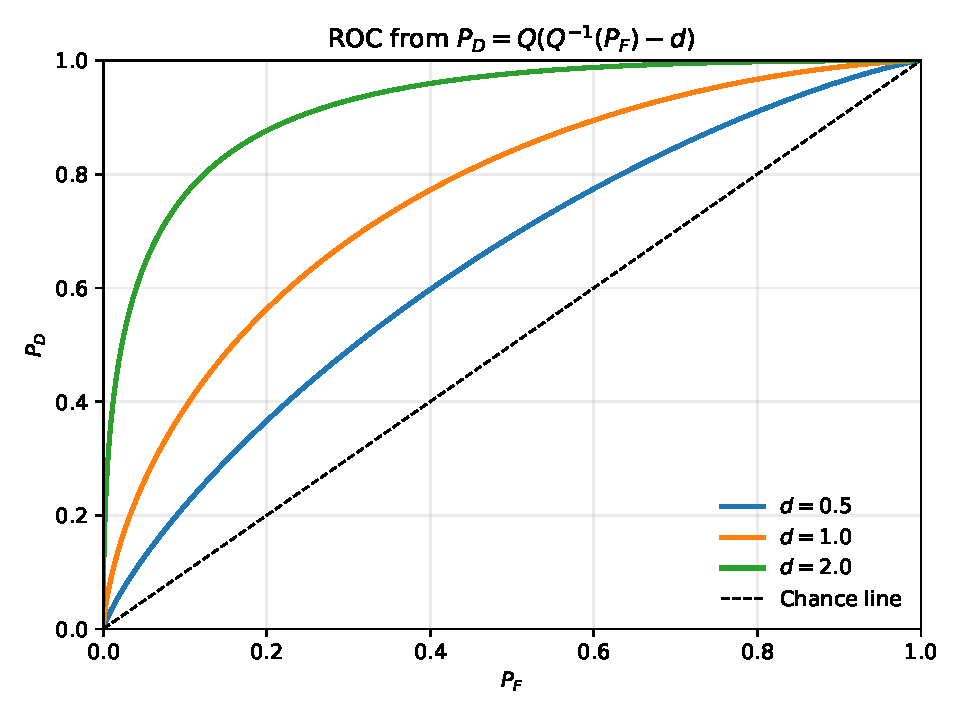
\includegraphics[width=0.62\textwidth]{q1c_roc.pdf}
    \caption{ROC curves from $P_D=Q(Q^{-1}(P_F)-d)$ for different $d$.}
    \label{fig:q1c_roc}
\end{figure}

\end{solution}

%----------------------------------------------------------------------
\questionheader{Problem 2}
%----------------------------------------------------------------------

\begin{solution}

\textbf{(a)}

Total area $=c\times 12$.

For pdf,
\[
12c=1\quad\Rightarrow\quad c=\frac{1}{12}.
\]

\[
P(H_0)=P(H_1)=\frac{1}{2}.
\]

\textbf{(b)}

\[
f(y,x\le 0)=f(y,H_0)=f(y\mid H_0)P(H_0)
\Rightarrow f(y\mid H_0)=2f(y,H_0).
\]

For $x\le 0$,
\[
\begin{aligned}
0\le y\le 2 &\quad\text{with value }\frac{1}{12}\times 2=\frac{1}{6},\\
-2\le y<0 &\quad\text{with value }\frac{1}{12}\times 2=\frac{1}{6},\\
1\le y\le 2 &\quad\text{with value }\frac{1}{12}\times 2=\frac{1}{6},\\
-2\le y\le -1 &\quad\text{with value }\frac{1}{12}\times 2=\frac{1}{6}.
\end{aligned}
\]

Hence,
\[
f(y\mid H_0)=
\begin{cases}
\dfrac{1}{3}, & -2\le y\le -1\ \text{or}\ 1\le y\le 2,\\[4pt]
\dfrac{1}{6}, & -1\le y\le 1,\\[4pt]
0, & \text{otherwise.}
\end{cases}
\]

For $x>0$,
\[
\begin{aligned}
0\le y\le 2 &\quad\text{with value }\frac{1}{12}\times 2=\frac{1}{6},\\
-2\le y\le 0 &\quad\text{with value }\frac{1}{12}\times 2=\frac{1}{6},\\
0\le y\le 1 &\quad\text{with value }\frac{1}{12}\times 2=\frac{1}{6},\\
-1\le y\le 0 &\quad\text{with value }\frac{1}{12}\times 2=\frac{1}{6}.
\end{aligned}
\]

Hence,
\[
f(y\mid H_1)=
\begin{cases}
\dfrac{1}{6}, & -2\le y\le -1\ \text{or}\ 1\le y\le 2,\\[4pt]
\dfrac{1}{3}, & -1\le y\le 1,\\[4pt]
0, & \text{otherwise.}
\end{cases}
\]

\begin{figure}[H]
    \centering
    \begin{minipage}{0.48\textwidth}
        \centering
        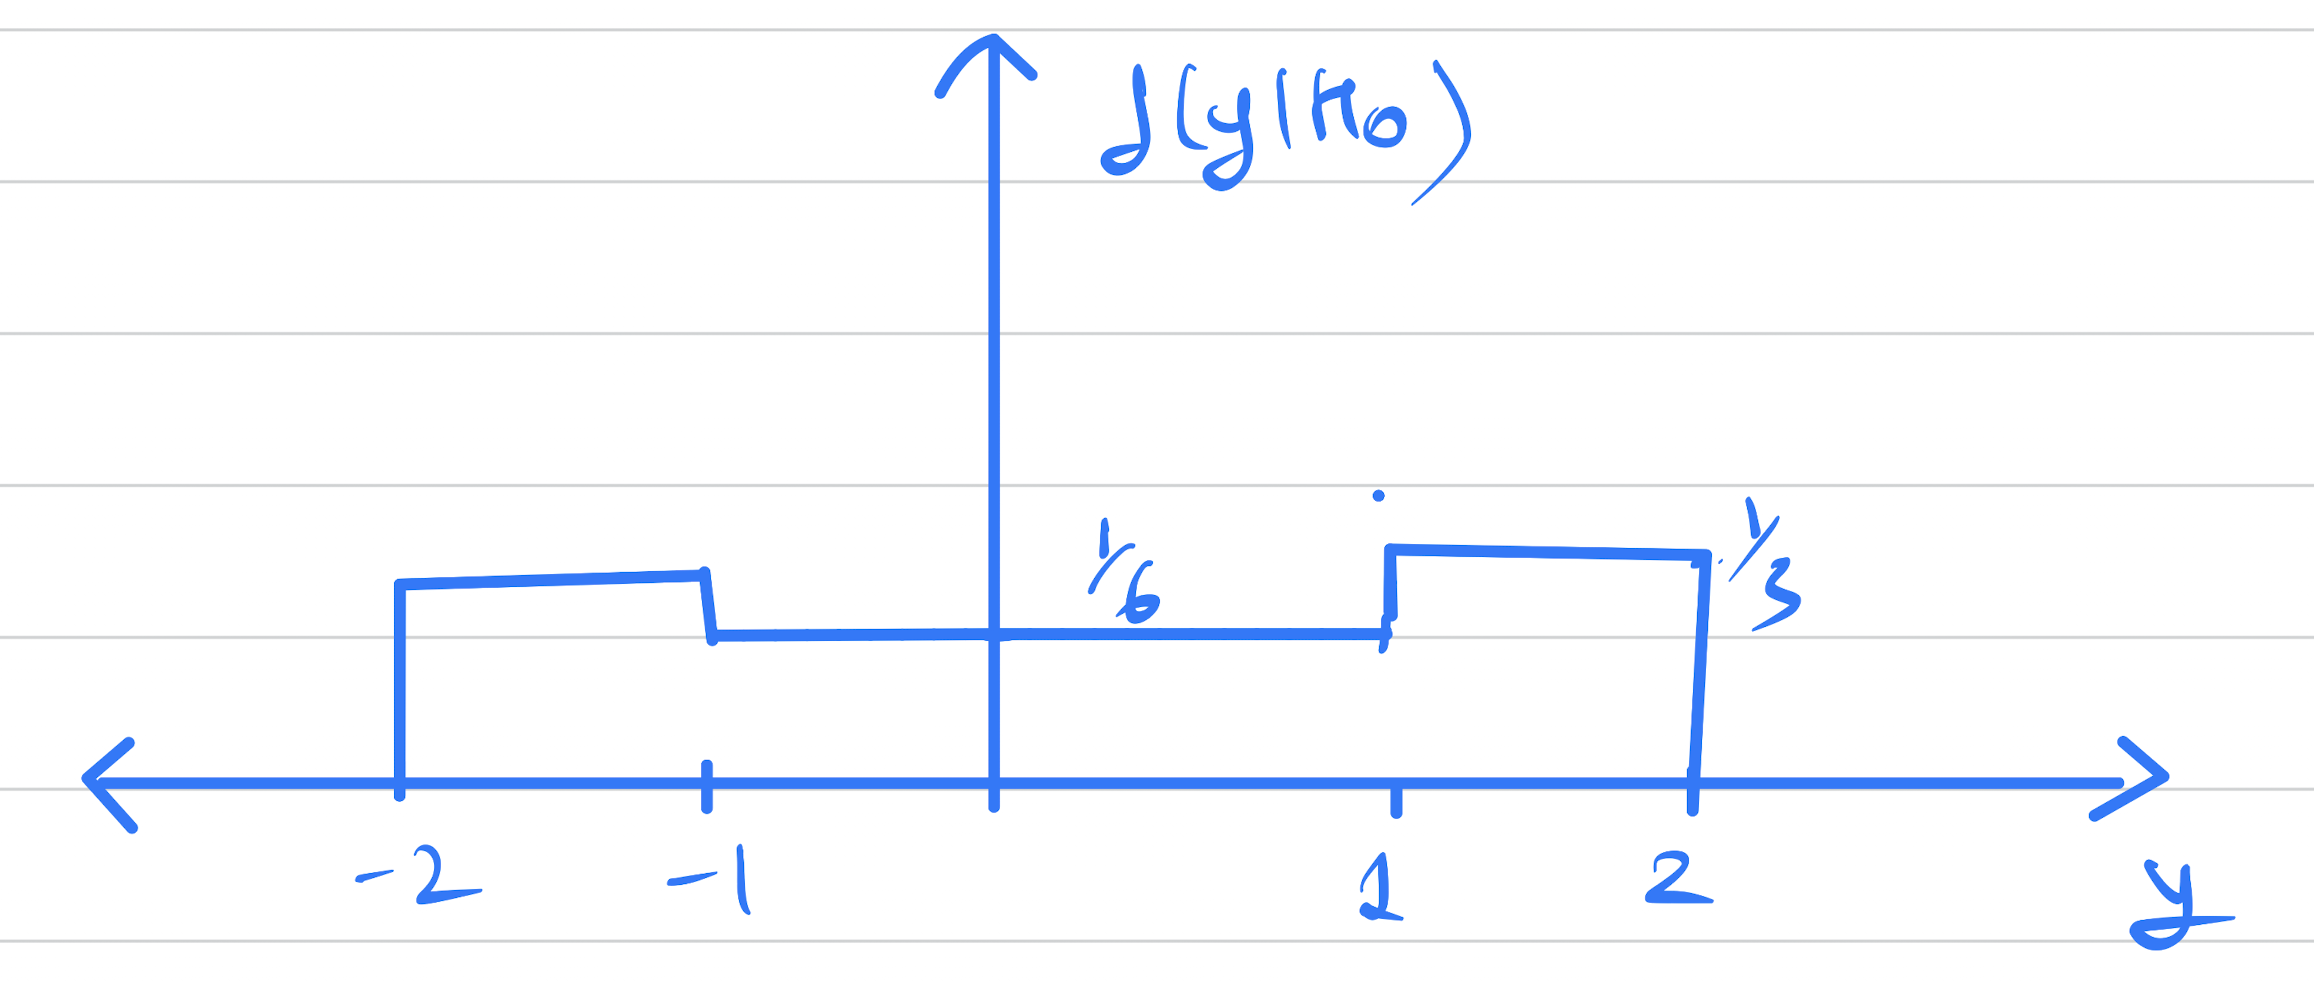
\includegraphics[width=\textwidth]{p2b_h0.png}
    \end{minipage}
    \hfill
    \begin{minipage}{0.48\textwidth}
        \centering
        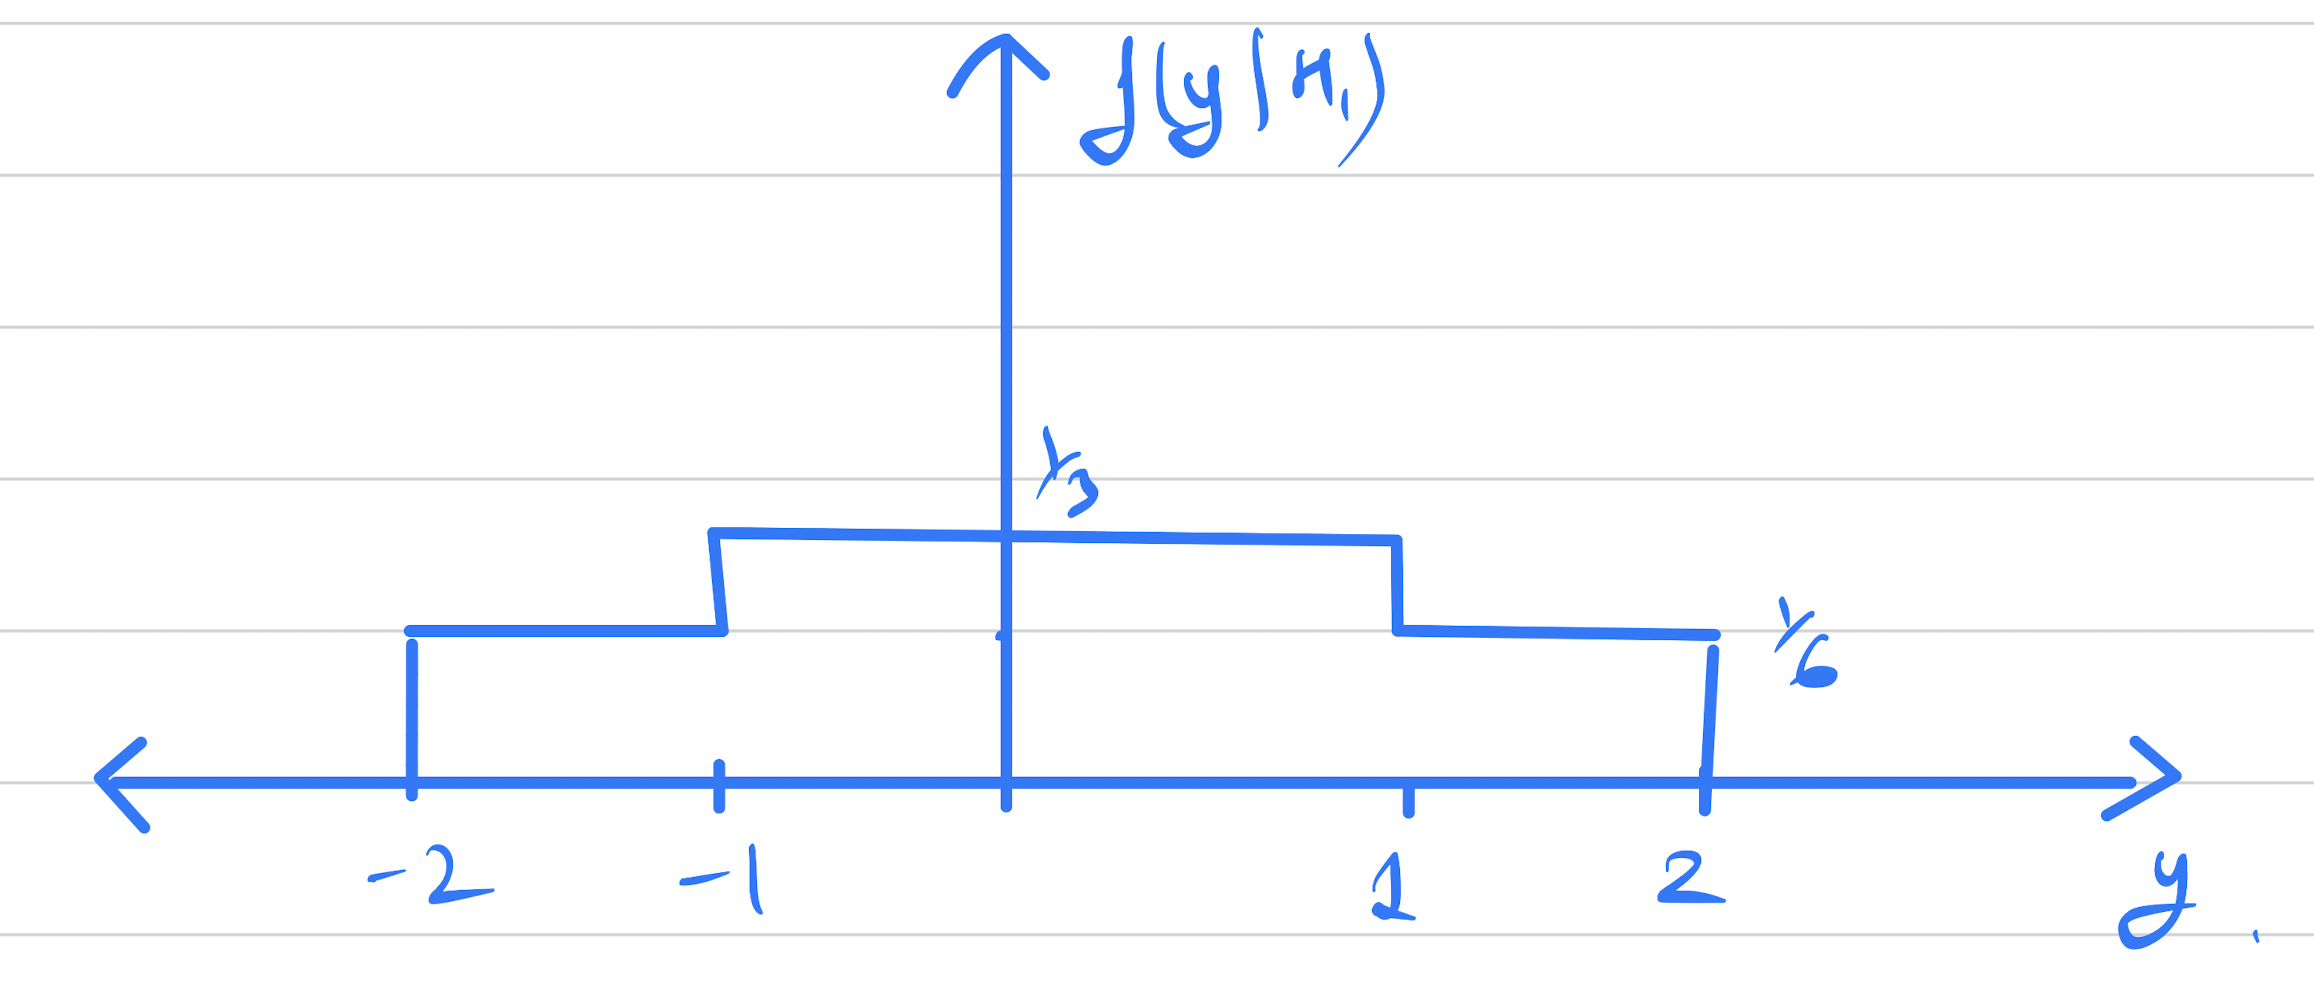
\includegraphics[width=\textwidth]{p2b_h1.png}
    \end{minipage}
    \caption{Sketches of $f(y\mid H_0)$ and $f(y\mid H_1)$ for Problem 2(b).}
    \label{fig:p2b_placeholders}
\end{figure}

\textbf{(c)}

\[
L(y)=\frac{f(y\mid H_1)}{f(y\mid H_0)}.
\]

\[
-1\le y\le 1:\quad L(y)=\frac{1/3}{1/6}=2,
\]
\[
1\le y\le 2\ \text{and}\ -2\le y\le -1:\quad L(y)=\frac{1/6}{1/3}=\frac{1}{2}.
\]

For uniform cost, decision rule
\[
L(y)\underset{H_0}{\overset{H_1}{\gtrless}}1.
\]

So,
\[
\delta(y)=
\begin{cases}
H_1, & -1\le y\le 1,\\
H_0, & 1\le y\le 2\ \text{and}\ -2\le y\le -1.
\end{cases}
\]

\textbf{(d)}

\[
P(\text{error})=P(H_1\mid H_0)P(H_0)+P(H_0\mid H_1)P(H_1)
\]
\[
=\frac{1}{2}\int_{-1}^{1}f(y\mid H_0)\,dy
+\frac{1}{2}\cdot 2\int_{1}^{2}f(y\mid H_1)\,dy
\quad [f(y\mid H_1)\ \text{is even}]
\]
\[
=\frac{1}{6}+\frac{1}{6}=\frac{1}{3}.
\]

\enlargethispage{12pt}
\end{solution}

%----------------------------------------------------------------------
\questionheader{Problem 3}
%----------------------------------------------------------------------

\begin{solution}

\[
\mathbf{y}=\begin{bmatrix}y_1\\y_2\\\vdots\\y_d\end{bmatrix},
\quad H_j,\ j=0,1,\dots,M-1,
\quad p_{ij}=\Pr\{y_i=1\mid H_j\}.
\]

\textbf{(a)}

\[
f(\mathbf{y}\mid H_j)=\prod_{i=1}^{d} f(y_i\mid H_j)
=\prod_{i=1}^{d} p_{ij}^{y_i}(1-p_{ij})^{1-y_i}
\quad [\text{independent}].
\]

Define
\[
f_j(\mathbf{y})=\ln\big(f(\mathbf{y}\mid H_j)P(H_j)\big)
=\sum_{i=1}^{d} y_i\ln\frac{p_{ij}}{1-p_{ij}}
+\sum_{i=1}^{d}\ln(1-p_{ij})
+\ln P(H_j).
\]

So,
\[
f(\mathbf{y}\mid H_j)P(H_j)\propto e^{f_j(\mathbf{y})}.
\]

\[
\Pr(\text{Error})=\Pr(\delta(\mathbf{y})\ne H)
=\sum_{j=0}^{M-1}\sum_{i=0,\,i\ne j}^{M-1}\Pr(\hat{H}=H_i, H=H_j)
\]
\[
=\sum_{j=0}^{M-1}\left(1-\Pr(\hat{H}=H_j, H=H_j)\right).
\]

In order to minimize $\Pr(\text{Error})$, we need to maximize
\[
\sum_{j=0}^{M-1}\Pr(\hat{H}=H_j, H=H_j)
=\max\sum_{j=0}^{M-1}\int_{Z_j} f(\mathbf{y}\mid H_j)P(H_j)\,d\mathbf{y}
\]
\[
=\max\left(\int_{Z_0}e^{f_0(\mathbf{y})}d\mathbf{y}+\int_{Z_1}e^{f_1(\mathbf{y})}d\mathbf{y}+\cdots+\int_{Z_{M-1}}e^{f_{M-1}(\mathbf{y})}d\mathbf{y}\right).
\]

Choose regions:
\[
Z_0=\{\mathbf{y}: f_0(\mathbf{y})\ge f_i(\mathbf{y})\ \forall i\ne 0\},
\]
\[
Z_1=\{\mathbf{y}: f_1(\mathbf{y})\ge f_i(\mathbf{y})\ \forall i\ne 1\},
\]
\[
\vdots
\]
\[
Z_{M-1}=\{\mathbf{y}: f_{M-1}(\mathbf{y})\ge f_i(\mathbf{y})\ \forall i\ne M-1\}.
\]

So, assign $H_j$ as
\[
j=\arg\max_j f_j(\mathbf{y}).
\]
That is the decision rule given in the question.

\textbf{(b)}

If $M=2$, $d$ be odd, $P(H_0)=P(H_1)=0.5$.

Decision rule reduces to
\[
\delta(\mathbf{y})=
\begin{cases}
H_1, & f_1(\mathbf{y})>f_0(\mathbf{y}),\\
H_0, & f_0(\mathbf{y})>f_1(\mathbf{y}).
\end{cases}
\]

Now $f_1(\mathbf{y})>f_0(\mathbf{y})$ gives
\[
\begin{aligned}
\sum_{i=1}^{d} y_i\ln\frac{p_{i1}}{1-p_{i1}}
+\sum_{i=1}^{d}\ln(1-p_{i1})
+\ln P(H_1)
&>
\sum_{i=1}^{d} y_i\ln\frac{p_{i0}}{1-p_{i0}}\\
&\quad
+\sum_{i=1}^{d}\ln(1-p_{i0})
+\ln P(H_0).
\end{aligned}
\]

With $p_{i0}=p$, $p_{i1}=1-p$,
\[
\sum_{i=1}^{d}y_i\left[\ln\frac{1-p}{p}-\ln\frac{p}{1-p}\right]
+\sum_{i=1}^{d}[\ln p-\ln(1-p)]>0.
\]

\[
\Rightarrow\quad 2\ln\frac{1-p}{p}\sum_{i=1}^{d}y_i > d\ln\frac{1-p}{p}.
\]

Since $p<\tfrac{1}{2}$,
\[
\sum_{i=1}^{d}y_i > \frac{d}{2}.
\]

So $H_1$ is decided when $\sum_{i=1}^{d}y_i>\frac{d}{2}$, $H_0$ otherwise.

\textbf{(c)}

\[
P_e=P(H_0\mid H_1)P(H_1)+P(H_1\mid H_0)P(H_0)
\]
\[
=\sum_{\sum y_i\le d/2}\Pr(\mathbf{y}\mid H_1)P(H_1)
+\sum_{\sum y_i> d/2}\Pr(\mathbf{y}\mid H_0)P(H_0).
\]

\[
\Pr(\mathbf{y}\mid H_0)=\prod_{i=1}^{d}\Pr(y_i\mid H_0)
=\prod_{i=1}^{d}p^{y_i}(1-p)^{1-y_i}
= p^{\sum y_i}(1-p)^{d-\sum y_i}.
\]

Summing Bernoulli independent trials is Binomial distribution.

So second term becomes
\[
\sum_{k=d/2+1}^{d} \binom{d}{k} p^k(1-p)^{d-k}.
\]

First term is
\[
\sum_{k=0}^{d/2} \binom{d}{k}(1-p)^k p^{d-k}.
\]

Both are basically the same term, so
\[
P(\text{error})
=\frac{1}{2}\sum_{k=0}^{d/2}\binom{d}{k}(1-p)^k p^{d-k}
+\frac{1}{2}\sum_{k=0}^{d/2}\binom{d}{k}(1-p)^k p^{d-k}
\]
\[
=\sum_{k=0}^{d/2}\binom{d}{k}(1-p)^k p^{d-k}.
\]

\end{solution}

%----------------------------------------------------------------------
\questionheader{Problem 4}
%----------------------------------------------------------------------

\begin{solution}

\[
H_k:\ Y\sim\text{Poisson}((k+1)\lambda),\quad k=0,1,2,\dots,M-1.
\]

\textbf{(a)}

Optimal Bayes test for $M$-ary with uniform cost and equal priors is ML detector.

\[
\hat{k}=\arg\max_{k\in\{0,1,\dots,M-1\}} f(y\mid H_k).
\]

Here,
\[
f(y\mid H_i)=\frac{e^{-(i+1)\lambda}((i+1)\lambda)^y}{y!}.
\]

So,
\[
\delta(y)=
\begin{cases}
H_0, & \text{if } f(y\mid H_0)\ge f(y\mid H_i)\ \forall i\ne 0,\\
H_1, & \text{if } f(y\mid H_1)\ge f(y\mid H_i)\ \forall i\ne 1,\\
\vdots\\
H_{M-1}, & \text{if } f(y\mid H_{M-1})\ge f(y\mid H_i)\ \forall i\ne M-1.
\end{cases}
\]

\textbf{(b)}

Pick up a decision region say $H_j$.

Then,
\[
f(y\mid H_j)\ge f(y\mid H_i),\quad \forall i\ne j.
\]

\[
\Rightarrow\quad
\frac{e^{-(j+1)\lambda}(j+1)^y\lambda^y}{y!}
\ge
\frac{e^{-(i+1)\lambda}(i+1)^y\lambda^y}{y!},\quad \forall i\ne j
\]

\[
\Rightarrow\quad
e^{-j\lambda}(j+1)^y\ge e^{-i\lambda}(i+1)^y
\]

\[
\Rightarrow\quad
-j\lambda+y\ln(j+1)\ge -i\lambda+y\ln(i+1)
\]

\[
\Rightarrow\quad
y\ln\frac{j+1}{i+1}\ge (j-i)\lambda
\]

\[
\Rightarrow\quad
y\ge \frac{(j-i)\lambda}{\ln\frac{j+1}{i+1}}.
\]

So, to decide $H_k$
\[
\frac{\lambda}{\ln\frac{k+2}{k+1}}\ge y\ge \frac{\lambda}{\ln\frac{k+1}{k}}.
\]

\textbf{(c)}

\[
P(\text{error})=\sum_{i=0}^{M-1}\Pr(\text{error}\mid H_i)P_i
=\sum_{i=0}^{M-1}\left[1-\Pr(H_i\mid H_i)\right]P_i.
\]

Now,
\[
\Pr(H_i\mid H_i)=
\sum_{y=\left\lceil \frac{\lambda}{\ln\frac{i+2}{i+1}}\right\rceil}^{\left\lfloor \frac{\lambda}{\ln\frac{i+1}{i}}\right\rfloor}
\frac{e^{-(i+1)\lambda}((i+1)\lambda)^y}{y!}.
\]

\[
P_i=\frac{1}{M}.
\]

\end{solution}

%----------------------------------------------------------------------
\questionheader{Problem 5}
%----------------------------------------------------------------------

\begin{solution}

\textbf{(a)}

For $y<0$,
\[
P_F=\int_{-\infty}^{0}\frac{1}{2}f(y\mid H_0)\,dy
=\frac{1}{2}\int_{-\infty}^{0}\frac{1}{2}e^{-|y|}\,dy
=\frac{1}{4}\int_{-\infty}^{0}e^y\,dy
=\frac{1}{4}.
\]

For $0\le y\le \tau$,
\[
P_F=\int_{0}^{\tau}\frac{1}{2}e^{-|y|}\,dy
=\frac{1}{2}(1-e^{-\tau}).
\]

For $y>\tau$, $P_F=0$.

For $y<0$,
\[
P_D=\frac{1}{2}\int_{-\infty}^{0}f(y\mid H_1)\,dy
=\frac{1}{2}\int_{-\infty}^{0}e^{-2|y|}\,dy
=\frac{1}{2}\int_{-\infty}^{0}e^{2y}\,dy
=\frac{1}{4}.
\]

For $0\le y\le \tau$,
\[
P_D=\int_{0}^{\tau}f(y\mid H_1)\,dy
=\int_{0}^{\tau}e^{-2|y|}\,dy
=\int_{0}^{\tau}e^{-2y}\,dy
=\frac{1-e^{-2\tau}}{2}.
\]

So,
\[
P_F=\frac{1}{4}+\frac{1}{2}(1-e^{-\tau}),
\qquad
P_D=\frac{1}{4}+\frac{1}{2}(1-e^{-2\tau}).
\]

\[
1-2\left(P_F-\frac{1}{4}\right)=e^{-\tau}.
\]

\[
\Rightarrow\quad
P_D=\frac{1}{4}+\frac{1}{2}\left[1-\left\{1-2\left(P_F-\frac{1}{4}\right)\right\}^2\right]
\]
\[
=\frac{1}{4}+2\left(P_F-\frac{1}{4}\right)-\left(P_F-\frac{1}{4}\right)^2.
\]

\begin{figure}[H]
    \centering
    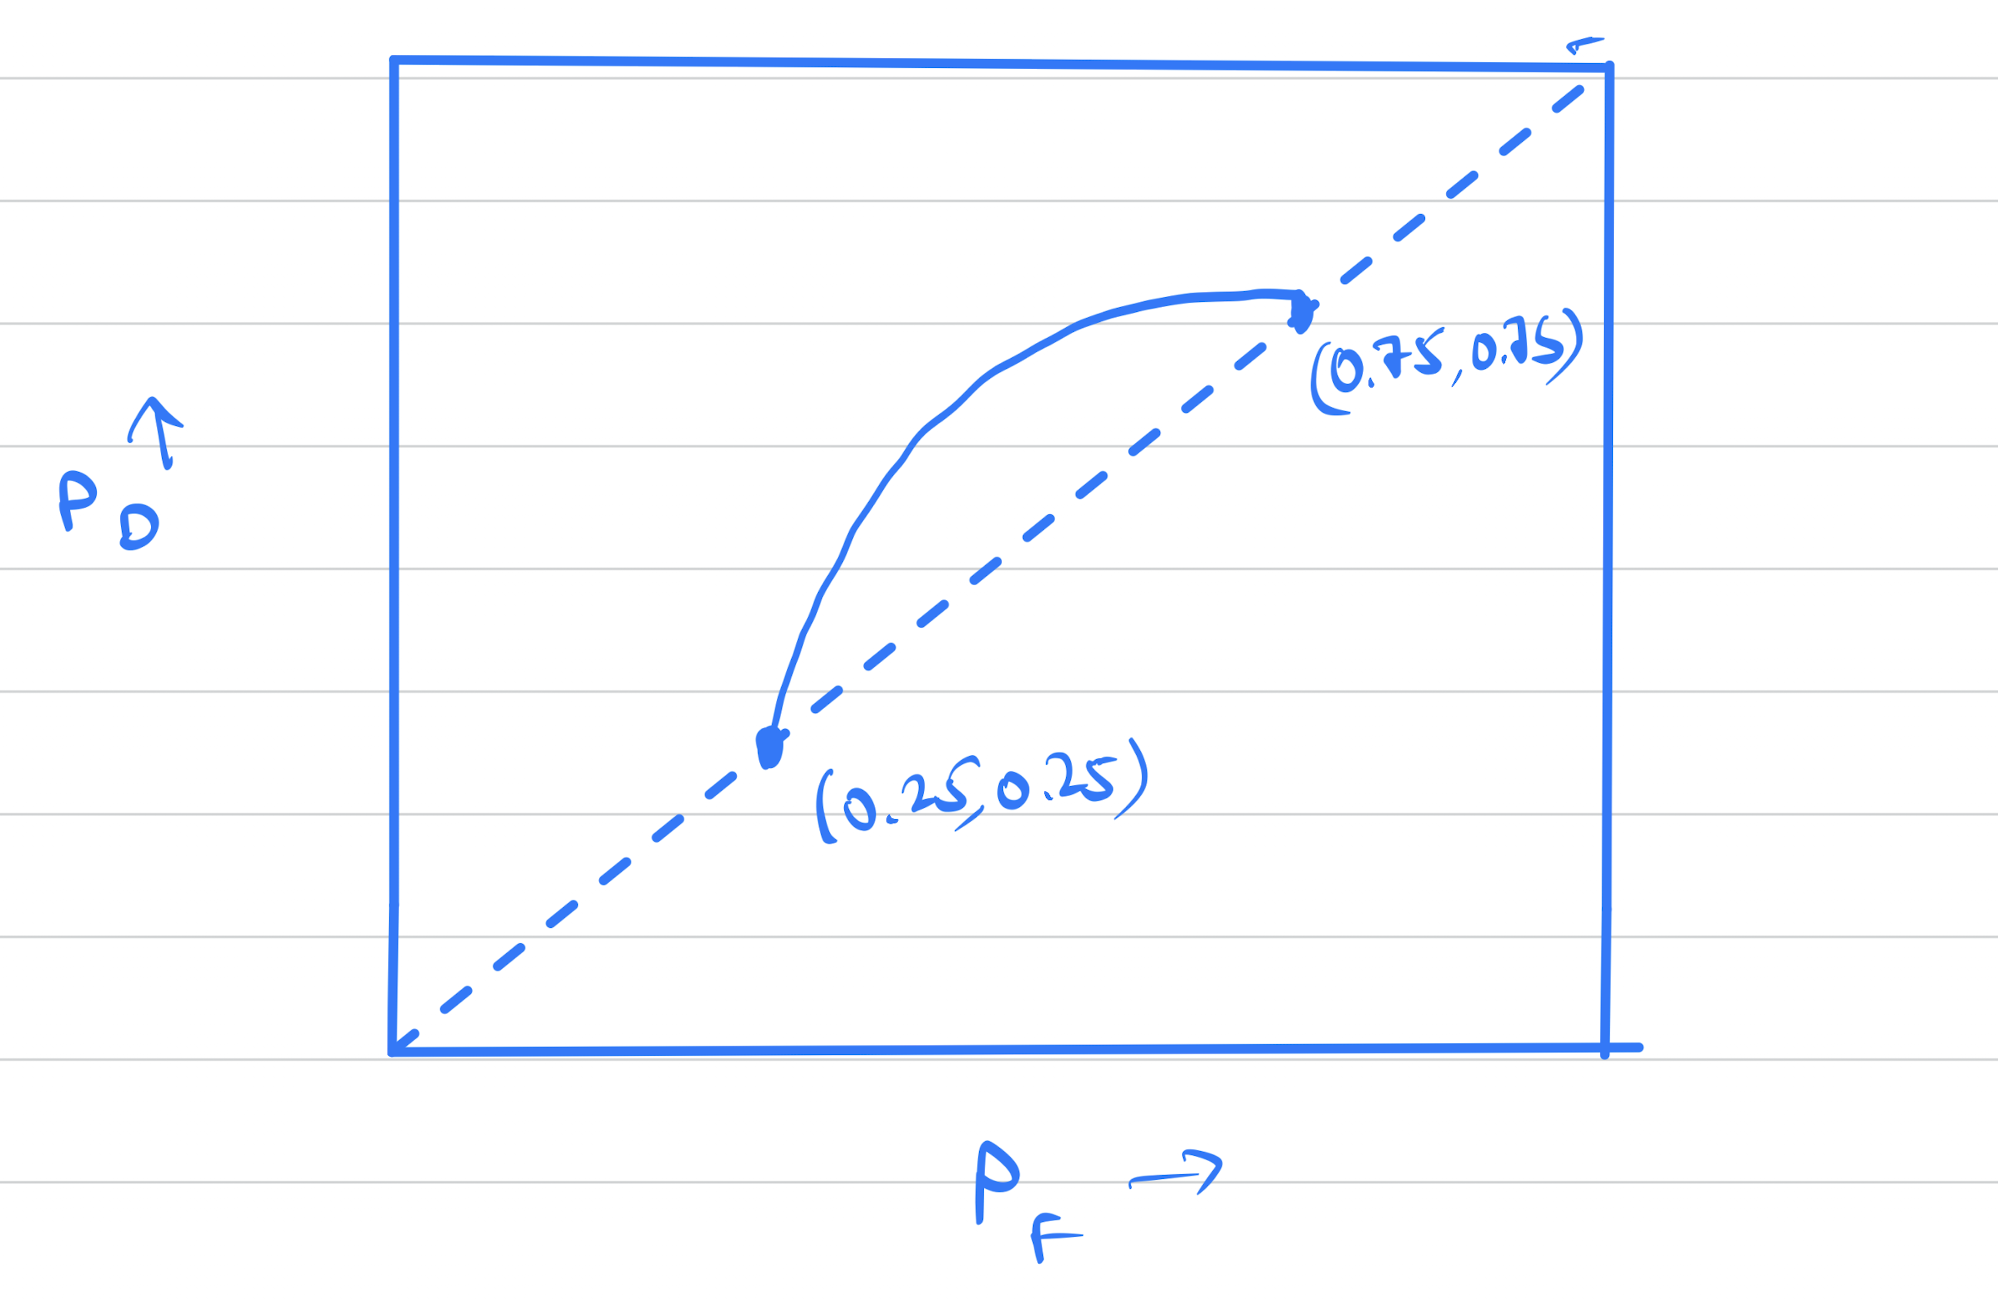
\includegraphics[width=0.62\textwidth]{P5a.png}
    \caption{ROC sketch for Problem 5(a).}
    \label{fig:p5a_placeholder}
\end{figure}

\textbf{(b)}

Let a randomization be defined between $(0,0)$ and $(\alpha,g(\alpha))$, where $(\alpha,g(\alpha))$ lies on ROC curve of $\delta_3(y)$.

Slope of the curve:
\[
\frac{dP_D}{dP_F}=\frac{dP_D}{d\tau}\cdot\frac{d\tau}{dP_F}
=\frac{e^{-2\tau}}{\frac{1}{2}e^{-\tau}}
=2e^{-\tau}.
\]

Slope of the line from origin:
\[
\frac{P_D}{P_F}=
\frac{\frac{3}{4}-\frac{1}{2}e^{-2\tau}}{\frac{3}{4}-\frac{1}{2}e^{-\tau}}.
\]

For tangency,
\[
\frac{P_D}{P_F}=\frac{dP_D}{dP_F}
\Rightarrow
\frac{\frac{3}{4}-\frac{1}{2}e^{-2\tau}}{\frac{3}{4}-\frac{1}{2}e^{-\tau}}=2e^{-\tau}.
\]

\[
\Rightarrow\quad
\frac{3}{4}-\frac{1}{2}e^{-2\tau}=\frac{3}{2}e^{-\tau}-e^{-2\tau}
\]
\[
\Rightarrow\quad
-\frac{1}{2}e^{-2\tau}-\frac{3}{2}e^{-\tau}+\frac{3}{4}=0
\]
\[
\Rightarrow\quad
e^{-2\tau}+3e^{-\tau}-1.5=0
\]
\[
\Rightarrow\quad
e^{-\tau}=\frac{1}{\sqrt{2}}.
\]

\[
\Rightarrow\quad
P_F=\frac{3}{4}-\frac{1}{2\sqrt{2}}=\frac{\sqrt{2}}{4}.
\]

This is the required $\alpha_0=\dfrac{\sqrt{2}}{4}$.

Similarly, by symmetry,
\[
\alpha_1=1-\alpha_0.
\]

\textbf{(c)}

We know from part (b),
\[
P_F\in[0,\alpha_0]\ \to\ \text{straight line (from randomization)}
\]
\[
P_F\in[\alpha_0,\alpha_1]\ \to\ \text{curve of }\delta_3
\]
\[
P_F\in[\alpha_1,1]\ \to\ \text{straight line (from randomization)}.
\]

\begin{figure}[H]
    \centering
    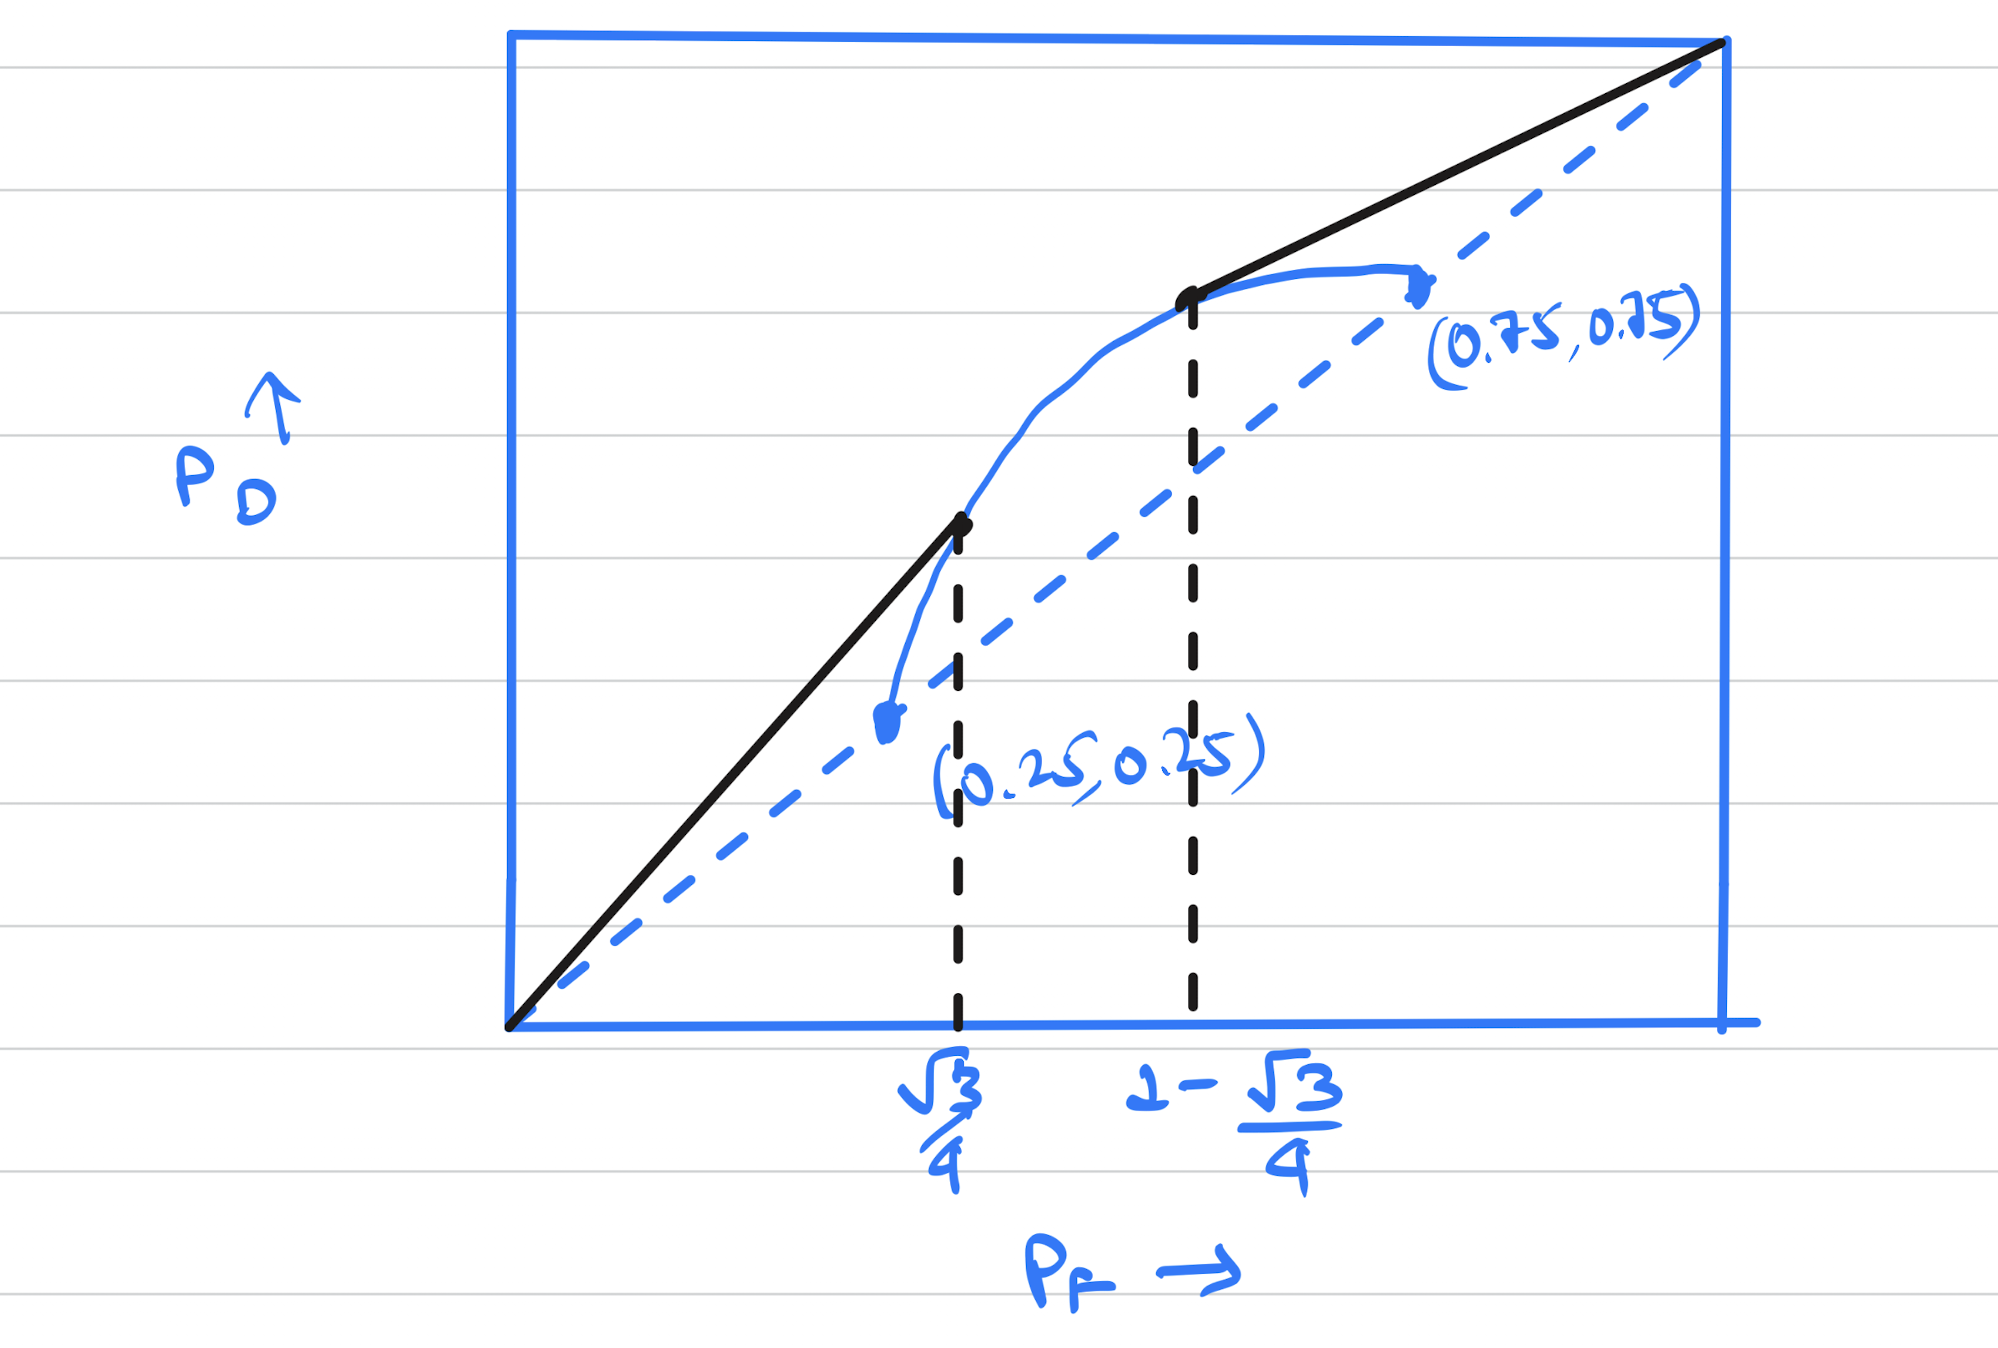
\includegraphics[width=0.62\textwidth]{P5c.png}
    \caption{ROC sketch for Problem 5(c).}
    \label{fig:p5c_placeholder}
\end{figure}

\end{solution}

\end{document}
